\item Consider the matrix $\vec{M} = \begin{pmatrix}2 & -1\\3 & 1\end{pmatrix}$. Which ONE of the following statements is TRUE?

	\hfill (DA 2024)
\begin{enumerate}
\item The eigenvalues of $\vec{M}$ are non-negative and real.
\item The eigenvalues of $\vec{M}$ are complex conjugate pairs.
\item One eigenvalue of $\vec{M}$ is positive and real, and another eigenvalue of $\vec{M}$ is zero.
\item One eigenvalue of $\vec{M}$ is non-negative and real, and another eigenvalue of $\vec{M}$ is negative and real.
\end{enumerate} 
\item Consider the dataset with six datapoints $\{\brak{\vec{x}_1, y_1}, \brak{\vec{x}_2, y_2}, \ldots, \brak{\vec{x}_6, y_6}\}$, where\\
$\vec{x}_1 = \myvec{1\\0}$,\quad $\vec{x}_2 = \myvec{0\\1}$,\quad $\vec{x}_3 = \myvec{0\\-1}$,\quad $\vec{x}_4 = \myvec{-1\\0}$,\quad $\vec{x}_5 = \myvec{2\\2}$,\quad $\vec{x}_6 = \myvec{-2\\-2}$,\\
and the labels are $y_1 = y_2 = y_5 = 1$ and $y_3 = y_4 = y_6 = -1$. A hard margin linear support vector machine is trained on the above dataset. Which ONE of the following sets is a possible set of support vectors?
	\hfill (DA 2024)
\begin{multicols}{2}
\begin{enumerate}
\item $\{\vec{x}_1, \vec{x}_2, \vec{x}_5\}$
\item $\{\vec{x}_3, \vec{x}_4, \vec{x}_5\}$
\item $\{\vec{x}_4, \vec{x}_5\}$
\item $\{\vec{x}_1, \vec{x}_2, \vec{x}_3, \vec{x}_4\}$
\end{enumerate} 
\end{multicols}
\item Euclidean distance based $k$-means clustering algorithm was run on a dataset of $100$ points with $k=3$. If the points $\myvec{1\\1}$ and $\myvec{-1\\1}$ are both part of cluster 3, then which ONE of the following points is necessarily also part of cluster 3?
	\hfill (DA 2024)
\begin{multicols}{4}
\begin{enumerate}
\item $\myvec{0\\0}$
\item $\myvec{0\\2}$
\item $\myvec{2\\0}$
\item $\myvec{0\\1}$
\end{enumerate} 
\end{multicols}
\item Consider the $3\times 3$ matrix
	$
\vec{M}=
\begin{pmatrix}
1 & 2 & 3\\
3 & 1 & 3\\
4 & 3 & 6
\end{pmatrix}
$.
The determinant of $\brak{\vec{M}^2 + 12\vec{M}}$ is \rule{8em}{0.07em}.
	\hfill (DA 2024)
\item Select all choices that are subspaces of $\mathbb{R}^3$.
	\hfill (DA 2024)
\begin{enumerate}
\item $\left\{\vec{x} = \begin{pmatrix}x_1\\x_2\\x_3\end{pmatrix} \in \mathbb{R}^3:\;\vec{x} = \alpha \begin{pmatrix}1\\1\\0\end{pmatrix}+\beta\begin{pmatrix}1\\0\\0\end{pmatrix}, \alpha, \beta\in \mathbb{R}\right\}$
\item $\left\{\vec{x} = \begin{pmatrix}x_1\\x_2\\x_3\end{pmatrix} \in \mathbb{R}^3:\;\vec{x} = \alpha^2 \begin{pmatrix}1\\2\\0\end{pmatrix}+\beta^2\begin{pmatrix}1\\0\\1\end{pmatrix}, \alpha, \beta\in \mathbb{R}\right\}$
\item $\left\{\vec{x} = \begin{pmatrix}x_1\\x_2\\x_3\end{pmatrix} \in \mathbb{R}^3:\;5x_1 + 2x_3 = 0,\, 4x_1-2x_2+3x_3=0\right\}$
\item $\left\{\vec{x} = \begin{pmatrix}x_1\\x_2\\x_3\end{pmatrix} \in \mathbb{R}^3:\;5x_1 + 2x_3 + 4 = 0\right\}$
\end{enumerate}
\item Which of the following statements is/are TRUE?
\begin{enumerate}
\item There exist $\vec{M} \in \mathbb{R}^{3\times3}$, $\vec{p} \in \mathbb{R}^3$, and $\vec{q} \in \mathbb{R}^3$ such that $\vec{M}\vec{x}=\vec{p}$ has a unique solution and $\vec{M}\vec{x}=\vec{q}$ has infinite solutions.
\item There exist $\vec{M} \in \mathbb{R}^{3\times3}$, $\vec{p} \in \mathbb{R}^3$, and $\vec{q} \in \mathbb{R}^3$ such that $\vec{M}\vec{x}=\vec{p}$ has no solutions and $\vec{M}\vec{x}=\vec{q}$ has infinite solutions.
\item There exist $\vec{M} \in \mathbb{R}^{2\times3}$, $\vec{p} \in \mathbb{R}^2$, and $\vec{q} \in \mathbb{R}^2$ such that $\vec{M}\vec{x}=\vec{p}$ has a unique solution and $\vec{M}\vec{x}=\vec{q}$ has infinite solutions.
\item There exist $\vec{M} \in \mathbb{R}^{3\times2}$, $\vec{p} \in \mathbb{R}^3$, and $\vec{q} \in \mathbb{R}^3$ such that $\vec{M}\vec{x}=\vec{p}$ has a unique solution and $\vec{M}\vec{x}=\vec{q}$ has no solutions.
\end{enumerate} 

\item Let $\mathbb{R}$ be the set of real numbers, $U$ be a subspace of $\mathbb{R}^3$ and $\vec{M} \in \mathbb{R}^{3\times 3}$ be the matrix corresponding to the projection onto the subspace $U$. Which of the following statements is/are TRUE?
	\hfill (DA 2024)
\begin{enumerate}
\item If $U$ is a $1$-dimensional subspace of $\mathbb{R}^3$, then the null space of $\vec{M}$ is a $1$-dimensional subspace.
\item If $U$ is a $2$-dimensional subspace of $\mathbb{R}^3$, then the null space of $\vec{M}$ is a $1$-dimensional subspace.
\item $\vec{M}^2 = \vec{M}$
\item $\vec{M}^3 = \vec{M}$
\end{enumerate} 

\item Let $\vec{u} = [1\ 2\ 3\ 4\ 5]^{\top}$, and let $\sigma_1, \sigma_2, \sigma_3, \sigma_4, \sigma_5$ be the singular values of the matrix $M = \vec{u} \vec{u}^{\top}$ where $\vec{u}^{\top}$ is the transpose of $\vec{u}$. The value of $\sum\limits_{i=1}^{5} \sigma_i$ is \rule{1cm}{0.01pt}.
	\hfill (DA 2024)
\item Given the two-dimensional dataset consisting of 5 data points from two classes (circles and squares) 
and using Euclidean distance as the metric, the minimum odd value of $k$ in the $k$-nearest neighbour algorithm  
for which the diamond ($\lozenge$) point is assigned the label ``square'' is \rule{1cm}{0.01pt}.
	\hfill (DA 2024)
\begin{figure}[H]
\centering
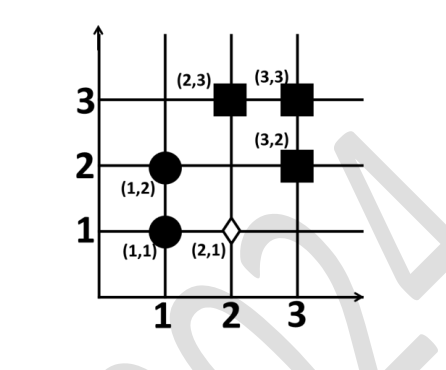
\includegraphics[width=0.45\columnwidth]{GATE/2024/DA/figs/63.png} % replace with actual KNN dataset figure
\label{fig:63}
\end{figure}

